\documentclass{article}
\usepackage{graphicx}
\usepackage{geometry}
\usepackage{hyperref}
\usepackage{mathtools}
\usepackage{float}
\usepackage{minted}
\graphicspath{{./}}
\geometry{a4paper, portrait, margin = 1in}
\title{2: Linear Regression in Pytorch, the Dumb Way}
\date{\today}
\author{Aniruddh K Budhgavi \\Enigma, IIIT-B}
\begin{document}
    \maketitle 
    \section{Introduction}
    Constructing machine learning models using Numpy is a fantastic way 
    of understanding the nitty-gritties of a particular method, but it is 
    not an ideal way for more complex models or in production environments.
    Instead, we use libraries like Pytorch, Tensorflow and Keras. These libraries
    ensure that you spend less time reinventing the wheel, leaving you free to fine-tune
    the model without getting bogged down by details. They also make your training process
    faster by utilizing the GPU (if you have one).
    \\
    My personal preference is towards Pytorch (anyone who has used Tensorflow 
    1.X will understand why). Pytorch has enough utilities to make the process painless
    but is flexible when it comes to customizations.
    \section{Installation}
    It is worth putting a separate section for this because of a few details. The primary
    complication is due to \textbf{CUDA}, a GPU computing API provided by NVIDIA. The GPU 
    implementation of Pytorch uses CUDA, so \textbf{you can only use Pytorch with a CUDA-
    capable NVIDIA GPU} (or any CPU). You can check if your GPU is supported at \url{https://developer.nvidia.com/cuda-gpus}.
    \\
    You can install Pytorch from \url{https://pytorch.org/get-started/locally/}. There are 
    various package managers and builds which are available.
    \begin{enumerate}
        \item On Windows, I recommend that you use the Anaconda package manager. Use the latest 
            stable version of Pytorch, and be sure to check the CUDA version (later the better).
        \item On Ubuntu, you can install using Pip without any troubles. \textbf{You may have to
        install CUDA manually}.To do so, visit \url{https://developer.nvidia.com/cuda-downloads}.
        \item In case your PC is underpowered, you can always run your models in Kaggle.
        In fact, that is what I do for Deep Learning models, even though I have a GTX 1050. 
        Kaggle provides (as of writing) 30 hrs per week of an NVIDIA Tesla P100 GPU. 
        You can even natively import Kaggle datasets without any trouble.
    \end{enumerate}
    To check if the installation was successful, open a Jupyter notebook and run:
    \begin{minted}{python}
        import torch
        torch.cuda.is_available()
    \end{minted}
    Expected output:
    \begin{minted}{python}
        True
    \end{minted}
    If the output doesn't match, you may have to manually install CUDA. Further, try:
    \begin{minted}{python}
        torch.cuda.get_device_name()
    \end{minted}
    Expected output should be something like:
    \begin{minted}{python}
        'GeForce GTX 1050'
    \end{minted}
    With this, we are ready to build a simple linear regression model using Pytorch.

    \begin{itemize}
        \item \textbf{Tip:} You can run Jupyter Notebooks in Visual Studio Code. This gives you 
        all of VS Code's syntax highlighting and autocomplete features. Just be sure to install 
        the Python plugin from the VS Code marketplace.
    \end{itemize}

    \section{Building the model}
    \begin{enumerate}
        \item You can find the code for this model \href{https://raw.githubusercontent.com/aniruddhkb/enigmatutorials/master/intro2ml/linearRegressionPytorch/linearRegressionTheDumbWay.ipynb}{here}.
        It won't make much sense in the browser -- download it and open in Jupyter.

        \item First, let us import the relevant libraries.
        \begin{minted}{python}
            import numpy as np 
            import torch 
            import matplotlib.pyplot as plt 
        \end{minted}
        \item Next, let's define a few helper functions.
        \begin{minted}{python}
            def forward(X, W, b):
                return W*X + b
            def mse(Yhat, Y, m):
                return (1/(2*m))*torch.sum((Yhat - Y)**2)
            def update(W, b, W_grad, b_grad, alpha):
                W = W -alpha*W_grad
                b = b - alpha*b_grad
                return W, b
        \end{minted}
        We use {\tt forward} to compute $\hat{Y}$. We use {\tt mse} 
        to compute $J$, the cost function. We use {\tt update} to update 
        the parameters $W$ and $b$.

        \item Next, let's define some hyperparameters.
        \begin{itemize}
            \item \emph{Hyperparameters} are those variables that you, the creator
            of the ML model specify in order to tune your model. This is in contrast
            to the model \emph{parameters}, which are learned through training.
            \item $W$ and $b$ are parameters, while $\alpha$ and $num\textunderscore iters$  are 
            hyperparameters.      
        \end{itemize}
        \begin{minted}{python}
            m = 100 # Number of data points.
            noise_qty = 0.1 # How noisy is the data to be generated?
            alpha = 0.0001 # The learning rate.
            num_iters = 100000 # The number of iterations.
        \end{minted}

        \item Next, let's generate the data.
        \begin{minted}{python}
            X = torch.rand(m)*m
            W_optim = torch.rand(1)
            b_optim = torch.rand(1)
            Y = forward(X, W_optim, b_optim) + torch.rand(m)*(m*noise_qty)
        \end{minted}
        \item Our dataset is $(X, Y)$. Let's plot it.
        \begin{minted}{python}
            plt.scatter(X, Y)
            plt.show()
        \end{minted}
        \begin{figure}[H] \begin{center}
            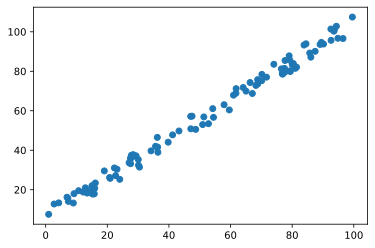
\includegraphics[width = 0.5\textwidth]{plot1.png}
            \caption{$Y$ as a function of $X$.}
        \end{center} \end{figure}

        \item Let's initialize $W$ and $b$.
        \begin{minted}{python}
            W = torch.rand(1, requires_grad=True)
            b = torch.rand(1, requires_grad=True)
        \end{minted}
        The argument \emph{requires\textunderscore grad = True} is needed for Pytorch's automatic 
        differentiation package. This tells Pytorch to maintain a record of the computational graph
        starting from these nodes. If this doesn't make sense, hold on.

        \item Let's visualize the current parameters.
        \begin{minted}{python}
            Yhat = forward(X, W, b).detach()
            plt.scatter(X, Y)
            plt.plot(X, Yhat, color = "red")
            plt.show()
        \end{minted}
        \begin{figure}[H] \begin{center}
            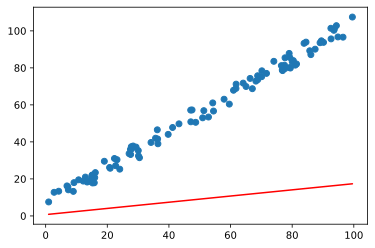
\includegraphics[width = 0.5\textwidth]{plot2.png}
            \caption{Our line, as expected.}
        \end{center} \end{figure}

        \item Now, we come to the key step of training. There are four steps:
        \begin{enumerate}
            \item Compute $\hat{Y}$.
            \item Compute $J(\hat(Y), Y)$, the cost function.
            \item Compute $\frac{\partial{J}}{\partial{W}}$ and $\frac{\partial{J}}{\partial{b}}$.
            \item Update $W$ and $b$.
        \end{enumerate}
        The code:
        \begin{minted}{python}
            costs = []
            for i in range(num_iters):
                if(i % (num_iters//100) == 0):
                    print("\r",i/(num_iters//100), "%", end = "")
                W = W.clone().detach().requires_grad_(True)
                b = b.clone().detach().requires_grad_(True)
                Yhat = forward(X, W, b)
                cost = mse(Yhat, Y, m)
                cost.backward()
                costs.append(cost.item())
                W, b = update(W, b ,W.grad, b.grad, alpha)
            print("")
        \end{minted}
        Let's go line by line.
        \begin{enumerate}
            \item The loop is the same as in Numpy.
            \item The {\tt if} block is to make a progress indicator.
            By using the escape sequence {\tt \textbackslash r}, we overwrite the previously printed number.
            \item I will explain {\tt W.clone} and {\tt b.clone} momentarily.
            \item The next two lines are to compute $\hat{Y}$ and $J$.
            \item This line is the deal-maker when it comes to Pytorch. 
            \begin{itemize}
                \item \textbf{Pytorch includes an automatic differentiation package called Autograd.}
                Using this, one can automatically compute the derivatives of a tensor with respect to other tensors.
                \item There are some preconditions as to which tensors can utilize Autograd.
                \item If you wish to compute the derivative of $b$ with respect to $a$, then, in the computation graph,
                \begin{enumerate}
                    \item $a$ must be a leaf node. What this means is that $a$ must not itself depend on some other tensors.
                    \item $a$ must be initialized with \tt{requires \textunderscore grad = True}.
                \end{enumerate}
                \item To compute $\frac{\partial{b}}{\partial{a}}$, first compute $b$ as a function of $a$, then run {\tt b.backward()}.
            \end{itemize}
            \item The next line {\tt update} is used to update $W$ and $b$.
        \end{enumerate}
        \item Now, we come to why we use \emph{W.clone} and \emph{b.clone}.
        \begin{enumerate}
            \item When we use tensors with {\tt requires\textunderscore grad = True}, Pytorch makes a \emph{computational graph} of the same and stores it.
            \item When we call {\tt tensor.backward()}, this computation graph is used to compute the derivatives.
            \item Here's the computational graph when we run {\tt cost.backward()} for the first time.
            \begin{figure}[H] \begin{center}
                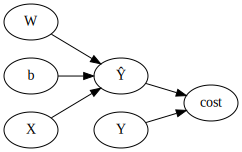
\includegraphics[width = 0.5\textwidth]{graph1.png}
            \end{center} \end{figure}
            \newpage
            \item Here's the computational graph when we run {\tt cost.backward()} for the second time.
            \begin{figure}[H] \begin{center}
                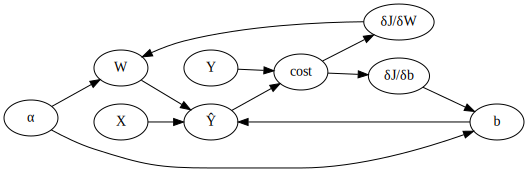
\includegraphics[width = \textwidth]{graph2.png}
            \end{center} \end{figure}
            Notice how, in the second graph, \textbf{$W$ and $b$ are no longer leaf nodes}. What this means
            is that {\tt W.grad} and {\tt b.grad} will both be {\tt None}. Further, we \emph{definitely} don't want 
            this kind of computational graph for {\tt cost.backward()}.
            \item The solution is to "refresh" $W$ and $b$ at each iteration.
        \end{enumerate}
        \item With that out of the way, let's see the plot for our new function.
        \begin{figure}[H] \begin{center}
            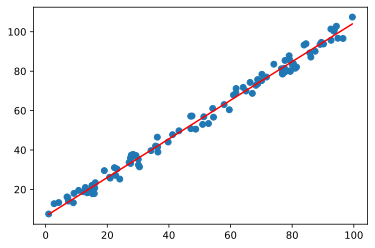
\includegraphics[width = 0.5\textwidth]{plot3.png}
        \end{center} \end{figure}
        \item And the cost:
        \begin{figure}[H] \begin{center}
            \includegraphics[width = 0.5\textwidth]{plot4.png}
        \end{center} \end{figure}  
    \end{enumerate}
    \newpage
    \section{Why was this the "dumb" way?}
    \begin{itemize}
        \item There are too many things that can go wrong here. 
        \item First, there's the business with refreshing $W$ and $b$ at every iteration.
        \item We could mess up the forward pass, the cost function or the update rule.
        \item Most importantly, here, we're reinventing the wheel. Pytorch has many utilities which make it 
        a very easy task to define and train models. 
        \item Imagine if we had to define the forward pass for a deep neural network or a convolutional neural network!
    \end{itemize}
    Next time, we'll see how we \emph{really} build and train models in Pytorch.
\end{document}